\documentclass[11pt, a4paper]{article}

% ── Codificação e idioma ──
\usepackage[utf8]{inputenc}
\usepackage[T1]{fontenc}
\usepackage[brazil]{babel}

% ── Layout ──
\usepackage[margin=1.8cm, top=2cm, bottom=1.8cm]{geometry}
\usepackage{enumitem}
\usepackage{multicol}

% ── Espaçamento ──
\setlength{\parskip}{2pt plus 1pt}
\setlength{\parindent}{0pt}

% ── Matemática ──
\usepackage{amsmath, amssymb}

% ── Tabelas e gráficos ──
\usepackage{booktabs}
\usepackage{array}
\usepackage{xcolor}
\usepackage{colortbl}
\usepackage{graphicx}
\usepackage[breakable]{tcolorbox}

% ── Cabeçalho e rodapé ──
\usepackage{fancyhdr}
\pagestyle{fancy}
\fancyhf{}
\lhead{\small Fundamentos de Sistemas Computacionais}
\rhead{\small Portas L\'{o}gicas e L\'{o}gica de Dois N\'{i}veis}
\cfoot{\thepage}
\renewcommand{\headrulewidth}{0.4pt}

% ── Configurações de listas ──
\setlist[enumerate,1]{label=\textbf{\arabic*.}, leftmargin=*, itemsep=4pt, topsep=4pt, parsep=1pt}
\setlist[enumerate,2]{label=\alph*), leftmargin=1.5em, itemsep=1pt, topsep=2pt, parsep=0pt}
\setlist[itemize]{itemsep=1pt, topsep=2pt, parsep=0pt}

% ── Caixas de destaque ──
\newtcolorbox{dica}{
  colback=blue!5!white,
  colframe=blue!50!black,
  title={\textbf{Dica}},
  fonttitle=\small,
  sharp corners,
  boxrule=0.5pt,
  left=4pt, right=4pt, top=2pt, bottom=2pt,
  before skip=4pt, after skip=4pt
}

\newtcolorbox{contexto}{
  colback=green!5!white,
  colframe=green!50!black,
  sharp corners,
  boxrule=0.5pt,
  left=4pt, right=4pt, top=3pt, bottom=3pt,
  before skip=4pt, after skip=4pt
}

\newtcolorbox{curiosidade}{
  colback=yellow!5!white,
  colframe=yellow!60!black,
  title={\textbf{Curiosidade}},
  fonttitle=\small,
  sharp corners,
  boxrule=0.5pt,
  left=4pt, right=4pt, top=2pt, bottom=2pt,
  before skip=4pt, after skip=4pt
}

% ══════════════════════════════════════════
\begin{document}

\begin{center}
  {\LARGE \textbf{Lista de Exerc\'{i}cios}}\\[4pt]
  {\Large Portas L\'{o}gicas e L\'{o}gica de Dois N\'{i}veis}\\[6pt]
  {\large 98800-04 -- Fundamentos de Sistemas Computacionais}\\[3pt]
  {\normalsize Prof.\ Ia\c{c}an\~{a} Ianiski Weber}
\end{center}

\vspace{2pt}
\hrule
\vspace{8pt}

\begin{enumerate}

% ── 1 ──
\item Complete as tabelas verdade para as portas AND, OR, NAND, NOR, XOR e XNOR de \textbf{2~entradas}, e para o inversor (NOT). Para cada uma, escreva a express\~{a}o booleana correspondente.

% ── 2 ──
\item Para cada descri\c{c}\~{a}o, identifique a porta l\'{o}gica:
\begin{enumerate}
  \item ``Sa\'{i}da~1 somente quando todas as entradas s\~{a}o~1.''
  \item ``Sa\'{i}da~1 quando pelo menos uma entrada \'{e}~1.''
  \item ``Sa\'{i}da~0 somente quando todas as entradas s\~{a}o~1.''
  \item ``Sa\'{i}da~1 quando as entradas s\~{a}o diferentes.''
  \item ``Sa\'{i}da~1 quando as entradas s\~{a}o iguais.''
  \item ``Sa\'{i}da~1 somente quando todas as entradas s\~{a}o~0.''
\end{enumerate}

% ── 3 ──
\item Construa a tabela verdade completa para cada porta de 3~entradas:
\begin{multicols}{2}
\begin{enumerate}
  \item $X = ABC$
  \item $X = A + B + C$
  \item $X = \overline{ABC}$
  \item $X = A \oplus B \oplus C$
\end{enumerate}
\end{multicols}

% ── 4 ──
\item Avalie as express\~{o}es abaixo para os valores indicados entre par\^{e}nteses $(A, B, C, \ldots)$.
\begin{multicols}{2}
\begin{enumerate}
  \item $X = AB + \overline{C}$ \quad $(1, 0, 1)$
  \item $X = \overline{A}B + A\overline{B}$ \quad $(1, 1)$
  \item $X = (A + B)\overline{C}$ \quad $(0, 1, 0)$
  \item $X = \overline{AB} + C$ \quad $(1, 1, 0)$
  \item $X = A(B + \overline{C}D)$ \quad $(1, 0, 1, 1)$
\end{enumerate}
\end{multicols}

% ── 5 ──
\item Dados os sinais de entrada $A$ e $B$ abaixo, desenhe a forma de onda da sa\'{i}da para cada porta indicada:
\begin{center}
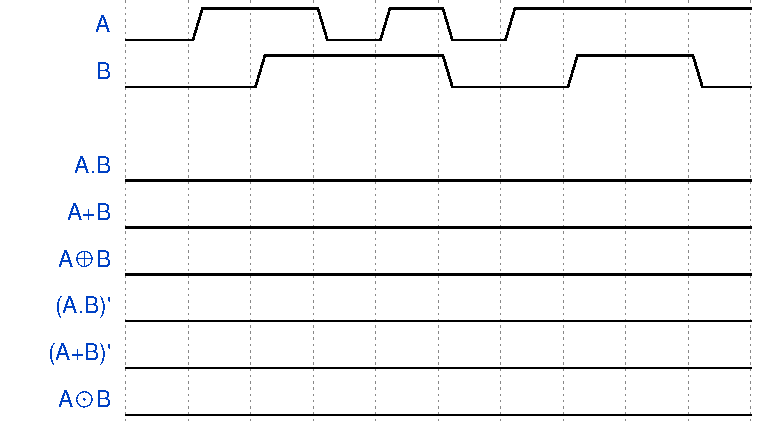
\includegraphics[width=0.85\textwidth]{img/q5_wavedrom.pdf}
\end{center}
% WaveDrom JSON (renderizar em https://wavedrom.com/editor.html e salvar como fig-q5-formas-de-onda.png):
% {signal: [
%   {name: 'A',    wave: '01.0101.'},
%   {name: 'B',    wave: '0.1..0.1'},
%   {},
%   {name: 'A.B',       wave: 'x.......'},
%   {name: 'A+B',       wave: 'x.......'},
%   {name: 'A⊕B',      wave: 'x.......'},
%   {name: '(A.B)\'',   wave: 'x.......'},
%   {name: '(A+B)\'',   wave: 'x.......'},
%   {name: 'A⊙B',      wave: 'x.......'}
% ]}

% ── 6: Equivalência / De Morgan ──
\item Usando tabelas verdade, verifique se os pares s\~{a}o equivalentes:
\begin{multicols}{2}
\begin{enumerate}
  \item $F_1 = A \oplus B$ \quad e \quad $F_2 = \overline{A}B + A\overline{B}$
  \item $F_1 = \overline{A+B}$ \quad e \quad $F_2 = \overline{A} \cdot \overline{B}$
  \item $F_1 = A + BC$ \quad e \quad $F_2 = (A+B)(A+C)$
  \item $F_1 = \overline{\overline{A} + \overline{B}}$ \quad e \quad $F_2 = AB$
\end{enumerate}
\end{multicols}

\newpage

% ── 7 ──
\item Para cada express\~{a}o, desenhe o circuito equivalente usando portas l\'{o}gicas:
\begin{multicols}{2}
\begin{enumerate}
  \item $X = \overline{A}B + A\overline{B}$
  \item $X = AB + C$
  \item $X = A\overline{B} + AB\overline{C}$
  \item $X = Z(X + \overline{X}\,\overline{Y})$
  \item $X = \overline{A + B} \cdot C$
  \item $X = (A + B + C)(\overline{A} + \overline{B} + C)$
\end{enumerate}
\end{multicols}

% ── 8: Circuito → Expressão ──
\item Para cada circuito descrito abaixo, determine a express\~{a}o booleana e construa a tabela verdade.

\begin{multicols}{2}
\begin{enumerate}
  \item Circuito:
  \begin{center}
    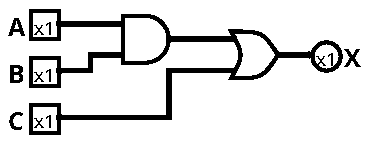
\includegraphics[width=0.35\textwidth]{img/q8a.pdf}
  \end{center}

  \item Circuito:
  \begin{center}
    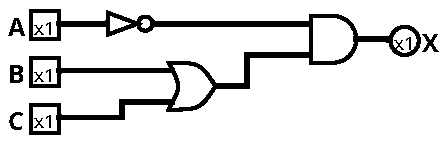
\includegraphics[width=0.35\textwidth]{img/q8b.pdf}
  \end{center}

  \item Circuito:
  \begin{center}
    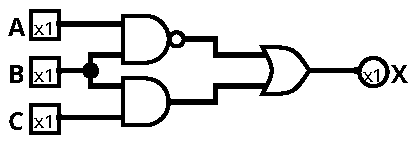
\includegraphics[width=0.35\textwidth]{img/q8c.pdf}
  \end{center}

  \item Circuito:
  \begin{center}
    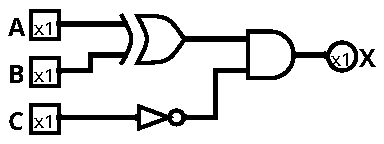
\includegraphics[width=0.35\textwidth]{img/q8d.pdf}
  \end{center}
\end{enumerate}
\end{multicols}

% ── 9: Tabela verdade → SOP/POS ──
\item Obtenha as express\~{o}es em SOP ($\Sigma$) e POS ($\Pi$) para cada tabela verdade:

\begin{multicols}{2}
\begin{enumerate}
\item ~

\begin{tabular}{ccc|c}
\toprule
$A$ & $B$ & $C$ & $F$ \\
\midrule
0 & 0 & 0 & 1 \\
0 & 0 & 1 & 0 \\
0 & 1 & 0 & 1 \\
0 & 1 & 1 & 0 \\
1 & 0 & 0 & 0 \\
1 & 0 & 1 & 1 \\
1 & 1 & 0 & 0 \\
1 & 1 & 1 & 1 \\
\bottomrule
\end{tabular}

\item ~

\begin{tabular}{ccc|c}
\toprule
$X$ & $Y$ & $Z$ & $S$ \\
\midrule
0 & 0 & 0 & 0 \\
0 & 0 & 1 & 1 \\
0 & 1 & 0 & 0 \\
0 & 1 & 1 & 1 \\
1 & 0 & 0 & 1 \\
1 & 0 & 1 & 0 \\
1 & 1 & 0 & 1 \\
1 & 1 & 1 & 0 \\
\bottomrule
\end{tabular}
\end{enumerate}
\end{multicols}

\noindent
\begin{minipage}[t]{0.48\textwidth}
\begin{enumerate}
\setcounter{enumii}{2}
\item[c)] ~

\begin{tabular}{cccc|c}
\toprule
$A$ & $B$ & $C$ & $D$ & $F$ \\
\midrule
0 & 0 & 0 & 0 & 0 \\
0 & 0 & 0 & 1 & 1 \\
0 & 0 & 1 & 0 & 0 \\
0 & 0 & 1 & 1 & 1 \\
0 & 1 & 0 & 0 & 0 \\
0 & 1 & 0 & 1 & 0 \\
0 & 1 & 1 & 0 & 1 \\
0 & 1 & 1 & 1 & 1 \\
1 & 0 & 0 & 0 & 0 \\
1 & 0 & 0 & 1 & 1 \\
1 & 0 & 1 & 0 & 0 \\
1 & 0 & 1 & 1 & 1 \\
1 & 1 & 0 & 0 & 1 \\
1 & 1 & 0 & 1 & 1 \\
1 & 1 & 1 & 0 & 1 \\
1 & 1 & 1 & 1 & 1 \\
\bottomrule
\end{tabular}
\end{enumerate}
\end{minipage}%
\hfill
\begin{minipage}[t]{0.48\textwidth}
\vspace{1.5em}
\begin{dica}
SOP $= \Sigma(...)$: \'{i}ndices das linhas onde $F=1$. \quad POS $= \Pi(...)$: \'{i}ndices das linhas onde $F=0$.
\end{dica}
\end{minipage}

\newpage
% ── 10: Conversões SOP/POS ──
\item Converta:
\begin{enumerate}
  \item $F(A,B,C) = \Sigma(0, 2, 5, 7)$ \quad $\rightarrow$ \quad $\Pi(?)$
  \item $G(X,Y,Z) = \Pi(1, 4, 6)$ \quad $\rightarrow$ \quad $\Sigma(?)$
  \item $H(A,B,C,D) = \Sigma(0, 1, 2, 5, 8, 9, 10)$ \quad $\rightarrow$ \quad $\Pi(?)$
\end{enumerate}

\vfill

% ── 11: Expansão para SOP canônica ──
\item Expanda para SOP can\^{o}nica (todos os mintermos expl\'{i}citos):
\begin{enumerate}
  \item $F = A + \overline{B}C$ \quad (vari\'{a}veis: $A$, $B$, $C$)
  \item $G = XY + Z$ \quad (vari\'{a}veis: $X$, $Y$, $Z$)
\end{enumerate}

\vfill

% ── 12: Análise completa ──
\item Considere: $F(A,B,C) = \overline{A}\,\overline{B}\,\overline{C} + A\overline{B}\,C + AB\overline{C} + ABC$
% DIAGRAMA SOP: 4 ANDs de 3 entradas (com inversores) → OR de 4 entradas
\begin{enumerate}
  \item Construa a tabela verdade.
  \item Expresse como $\Sigma$ e como $\Pi$.
  \item Escreva a express\~{a}o POS completa (maxtermos expl\'{i}citos).
  \item Desenhe o circuito na forma SOP (ANDs~+~OR).
  \item Desenhe o circuito na forma POS (ORs~+~AND).
\end{enumerate}

\vfill

% ── 13: Alarme residencial ──
\item Uma empresa de seguran\c{c}a contratou voc\^{e} para projetar o circuito l\'{o}gico do painel de alarme de uma resid\^{e}ncia. O sistema possui tr\^{e}s sensores:
\begin{itemize}
  \item $P$ = sensor magn\'{e}tico na \textbf{porta principal} (1 = porta aberta)
  \item $J$ = sensor na \textbf{janela} da sala (1 = janela aberta)
  \item $M$ = sensor \textbf{infravermelho} de movimento (1 = movimento detectado)
\end{itemize}
O alarme ($A$) deve disparar quando: (i)~porta e janela est\~{a}o abertas simultaneamente, \textbf{ou} (ii)~movimento \'{e} detectado com a porta aberta.
\begin{enumerate}
  \item Escreva a express\~{a}o booleana para $A$.
  \item Construa a tabela verdade completa.
  \item Expresse $A$ em SOP ($\Sigma$) e POS ($\Pi$).
  \item Projete o circuito usando portas l\'{o}gicas.
\end{enumerate}

\vfill

% ── 14: Esteira industrial ──
\item Voc\^{e} trabalha numa f\'{a}brica de autope\c{c}as e precisa projetar o circuito de parada de emerg\^{e}ncia de uma esteira transportadora. A esteira tem:
\begin{itemize}
  \item $E$ = bot\~{a}o f\'{i}sico de \textbf{emerg\^{e}ncia} (1 = pressionado)
  \item $T$ = sensor de \textbf{temperatura} no motor (1 = superaquecimento)
  \item $C$ = c\'{e}lula de \textbf{carga} na esteira (1 = sobrecarga)
\end{itemize}
A esteira deve \textbf{parar} ($S = 1$) se: (i)~o bot\~{a}o de emerg\^{e}ncia for pressionado, \textbf{ou} (ii)~superaquecimento e sobrecarga ocorrerem ao mesmo tempo.
\begin{enumerate}
  \item Escreva a express\~{a}o para $S$ e construa a tabela verdade.
  \item Projete o circuito.
  \item O gerente de produ\c{c}\~{a}o pede para incluir um quarto sensor $H$ (umidade excessiva). A esteira tamb\'{e}m deve parar se houver umidade \textbf{e} superaquecimento simult\^{a}neos. Atualize a express\~{a}o e o circuito.
\end{enumerate}

\vfill

% ── 15: Votação ──
\item Na assembleia geral de uma associa\c{c}\~{a}o profissional, 3~diretores ($A$, $B$ e $C$) votam propostas. Uma proposta \'{e} aprovada ($F = 1$) pela maioria (pelo menos 2 de 3 votos a favor).
\begin{enumerate}
  \item Construa a tabela verdade.
  \item Obtenha SOP e POS.
  \item Projete o circuito SOP.
  \item Se o comit\^{e} for ampliado para \textbf{4~membros} e a regra for maioria simples (pelo menos 3 de 4), quantos mintermos a SOP teria?
\end{enumerate}

\newpage
% ── 16: Airbag ──
\item Fabricantes de autom\'{o}veis utilizam l\'{o}gica combinacional para decidir se o airbag deve inflar. Em um modelo simplificado, os sensores s\~{a}o:
\begin{itemize}
  \item $I$ = aceler\^{o}metro frontal (1 = impacto detectado)
  \item $V$ = velocidade acima de 25\,km/h no instante do impacto (1 = sim)
  \item $O$ = sensor de presen\c{c}a no banco (1 = ocupante sentado)
  \item $D$ = chave de desativa\c{c}\~{a}o manual do airbag (1 = desativado)
\end{itemize}
O airbag infla ($A = 1$) quando \textbf{todas} as condi\c{c}\~{o}es seguintes s\~{a}o verdadeiras: impacto detectado, velocidade acima de 25\,km/h, ocupante presente e airbag \textbf{n\~{a}o} desativado.
\begin{enumerate}
  \item Escreva a express\~{a}o booleana para $A$.
  \item Construa a tabela verdade (16~linhas).
  \item Quantos mintermos $A$ possui? Expresse como $\Sigma$.
  \item Expresse como $\Pi$.
  \item Projete o circuito.
\end{enumerate}

% ── 17: Cofre bancário ──
\item Um cofre de ag\^{e}ncia banc\'{a}ria exige m\'{u}ltiplos mecanismos para abrir:
\begin{itemize}
  \item $K$ = chave f\'{i}sica inserida (1 = sim)
  \item $S$ = senha num\'{e}rica correta (1 = sim)
  \item $B$ = biometria validada (1 = sim)
\end{itemize}
O cofre abre ($F = 1$) quando a chave est\'{a} inserida \textbf{E} pelo menos uma das outras verifica\c{c}\~{o}es (senha ou biometria) \'{e} satisfeita.
\begin{enumerate}
  \item Escreva a express\~{a}o e construa a tabela verdade.
  \item Projete o circuito.
  \item O banco decide adicionar uma restri\c{c}\~{a}o temporal: fora do hor\'{a}rio comercial ($T=0$), o cofre s\'{o} abre se \textbf{todos os tr\^{e}s} mecanismos forem satisfeitos. Em hor\'{a}rio comercial ($T=1$), a regra original se mant\'{e}m. Escreva a nova express\~{a}o para $F$.
\end{enumerate}

% ── 18: Semáforo ──
\item A prefeitura est\'{a} testando sem\'{a}foros adaptativos em um cruzamento. Sensores indutivos no asfalto e bot\~{o}es para pedestres fornecem:
\begin{itemize}
  \item $V_1$ = ve\'{i}culos detectados na via principal (1 = sim)
  \item $V_2$ = ve\'{i}culos detectados na via secund\'{a}ria (1 = sim)
  \item $P$ = pedestre aguardando (1 = sim)
\end{itemize}
O sinal da via principal fica \textbf{verde} ($G = 1$) quando: (i)~h\'{a} ve\'{i}culos na via principal e n\~{a}o h\'{a} pedestres, \textbf{ou} (ii)~h\'{a} ve\'{i}culos na via principal e n\~{a}o h\'{a} ve\'{i}culos na secund\'{a}ria.
\begin{enumerate}
  \item Escreva a express\~{a}o para $G$ e construa a tabela verdade.
  \item Expresse em $\Sigma$ e $\Pi$.
  \item Projete o circuito SOP.
\end{enumerate}

% ── 19: Display 7 segmentos ──
\item Displays de 7~segmentos est\~{a}o em rel\'{o}gios digitais, pain\'{e}is de elevadores e bombas de gasolina. Cada segmento \'{e} uma fun\c{c}\~{a}o l\'{o}gica de 4~entradas BCD ($A_3 A_2 A_1 A_0$). Considere o \textbf{segmento~\texttt{a}} (horizontal superior), que acende para os d\'{i}gitos 0, 2, 3, 5, 6, 7, 8, 9.
\begin{enumerate}
  \item Construa a tabela verdade (16~linhas).
  \item Escreva a SOP considerando apenas os mintermos com sa\'{i}da~1.
  \item Expresse usando $\Sigma$.
\end{enumerate}

% ── 20: Comparador ──
\item Projete um circuito comparador que recebe dois bits $A$ e $B$ e produz:
\begin{itemize}
  \item $G = 1$ quando $A > B$
  \item $E = 1$ quando $A = B$
  \item $L = 1$ quando $A < B$
\end{itemize}
\begin{enumerate}
  \item Construa a tabela verdade (4 linhas, 3 sa\'{i}das).
  \item Escreva as express\~{o}es booleanas para $G$, $E$ e $L$.
  \item Identifique qual porta l\'{o}gica b\'{a}sica implementa $E$ diretamente.
  \item Projete o circuito completo.
\end{enumerate}

\newpage
% ── 21: Half adder ──
\item Um \emph{half adder} (meio-somador) \'{e} o bloco fundamental da aritm\'{e}tica dentro de processadores. Ele recebe dois bits $A$ e $B$ e produz a \textbf{soma} $S$ e o \textbf{carry} (\emph{vai-um}) $C_{\text{out}}$.
\begin{enumerate}
  \item Construa a tabela verdade.
  \item Escreva as express\~{o}es para $S$ e $C_{\text{out}}$.
  \item Identifique quais portas implementam $S$ e $C_{\text{out}}$.
  \item Projete o circuito.
\end{enumerate}

% ── 22: Paridade ──
\item Em protocolos como UART (\emph{Universal Asynchronous Receiver-Transmitter}), um bit de paridade \'{e} adicionado a cada byte transmitido para detectar erros. Projete um circuito que recebe 3~bits de dados ($D_2, D_1, D_0$) e gera um bit de paridade $P$ tal que o total de bits~1 (dados~+~$P$) seja sempre \textbf{par}.
\begin{enumerate}
  \item Construa a tabela verdade.
  \item Escreva a SOP para $P$.
  \item Qual porta l\'{o}gica implementa isso diretamente, encadeada?
  \item Se um dos 4~bits for corrompido na transmiss\~{a}o, o receptor detecta o erro? E se dois bits forem corrompidos?
\end{enumerate}

% ── 25: Data center ──
\item Voc\^{e} foi contratado para projetar o sistema de alertas de um data center. Quatro sensores monitoram o ambiente:
\begin{itemize}
  \item $T$ = temperatura acima do limite (1 = sim)
  \item $U$ = umidade acima do limite (1 = sim)
  \item $R$ = falha no sistema de refrigera\c{c}\~{a}o (1 = sim)
  \item $E$ = opera\c{c}\~{a}o com gerador de emerg\^{e}ncia (1 = sim)
\end{itemize}
O sistema emite \textbf{alerta cr\'{i}tico} ($C = 1$) quando:
\begin{itemize}
  \item Temperatura alta \textbf{com} falha na refrigera\c{c}\~{a}o, \textbf{ou}
  \item Opera\c{c}\~{a}o com gerador e \textbf{qualquer} outra anomalia ($T$, $U$ ou $R$), \textbf{ou}
  \item Tr\^{e}s ou mais condi\c{c}\~{o}es anormais simult\^{a}neas.
\end{itemize}
\begin{multicols}{2}
\begin{enumerate}
  \item Modele cada condi\c{c}\~{a}o como express\~{a}o booleana separada.
  \item Combine numa express\~{a}o \'{u}nica para $C$.
  \item Construa a tabela verdade (16~linhas).
  \item Expresse $C$ em $\Sigma$.
\end{enumerate}
\end{multicols}

% ── 26: Multiplexador ──
\item Multiplexadores est\~{a}o em todo lugar: sele\c{c}\~{a}o de registradores na CPU, roteamento de redes, seletores de entrada de \'{a}udio/v\'{i}deo. Um mux 2:1 tem entradas de dados $D_0$, $D_1$, sele\c{c}\~{a}o $S$, e sa\'{i}da $Y$. Se $S=0$, $Y=D_0$; se $S=1$, $Y=D_1$.
\begin{enumerate}
  \item Construa a tabela verdade (8~linhas).
  \item Obtenha a SOP e simplifique para $Y = \overline{S} \cdot D_0 + S \cdot D_1$.
  \item Projete o circuito.
\end{enumerate}

% ── 27: Decodificador ──
\item Decodificadores s\~{a}o a base do endere\c{c}amento de mem\'{o}ria: quando a CPU envia um endere\c{c}o de 2~bits, o decodificador seleciona qual das 4~c\'{e}lulas de mem\'{o}ria ser\'{a} acessada. Entradas $A_1, A_0$; sa\'{i}das $Y_0, Y_1, Y_2, Y_3$ (exatamente uma ativa por vez).
\begin{enumerate}
  \item Construa a tabela verdade.
  \item Escreva a express\~{a}o para cada sa\'{i}da $Y_i$.
  \item Projete o circuito.
  \item Que rela\c{c}\~{a}o cada sa\'{i}da $Y_i$ tem com os \textbf{mintermos} de $A_1, A_0$?
\end{enumerate}

% ── 28: Validador de código ──
\item Uma empresa de seguran\c{c}a usa cart\~{o}es magn\'{e}ticos que codificam um valor de 4~bits ($A_3 A_2 A_1 A_0$). S\~{a}o considerados v\'{a}lidos \textbf{apenas} os c\'{o}digos com \textbf{exatamente dois bits em~1}: $0011$, $0101$, $0110$, $1001$, $1010$, $1100$.
\begin{enumerate}
  \item Construa a tabela verdade (16~linhas).
  \item Expresse $F$ em $\Sigma$ e $\Pi$.
  \item O que todos os c\'{o}digos v\'{a}lidos t\^{e}m em comum? Qual padr\~{a}o combinat\'{o}rio isso representa?
  \item Quantos c\'{o}digos v\'{a}lidos existiriam se o cart\~{a}o usasse 5~bits, com a mesma regra?
\end{enumerate}

% ── 29: Desafio final ──
\item Uma propriedade rural utiliza sensores para decidir quando irrigar automaticamente:
\begin{itemize}
  \item $S$ = umidade do solo abaixo do m\'{i}nimo (1 = solo seco)
  \item $C$ = previs\~{a}o de chuva nas pr\'{o}ximas 6h (1 = chuva prevista)
  \item $N$ = hor\'{a}rio noturno, quando a evapora\c{c}\~{a}o \'{e} menor (1 = noite)
  \item $R$ = reservat\'{o}rio de \'{a}gua com n\'{i}vel suficiente (1 = sim)
\end{itemize}
A irriga\c{c}\~{a}o \'{e} ativada ($I = 1$) quando:
\begin{itemize}
  \item O solo est\'{a} seco, \textbf{E}
  \item N\~{a}o h\'{a} previs\~{a}o de chuva, \textbf{E}
  \item O reservat\'{o}rio tem n\'{i}vel suficiente, \textbf{E}
  \item \'{E} hor\'{a}rio noturno.
\end{itemize}
Por\'{e}m, h\'{a} uma \textbf{exce\c{c}\~{a}o}: se o solo estiver seco \textbf{e} n\~{a}o houver previs\~{a}o de chuva \textbf{e} o reservat\'{o}rio tiver n\'{i}vel, a irriga\c{c}\~{a}o tamb\'{e}m \'{e} ativada durante o dia --- mas apenas nesse caso de urg\^{e}ncia h\'{i}drica.
\begin{enumerate}
  \item Escreva a express\~{a}o booleana para $I$.
  \item Construa a tabela verdade (16~linhas).
  \item Expresse em $\Sigma$ e $\Pi$.
  \item Projete o circuito.
\end{enumerate}

\end{enumerate}


\end{document}
